\documentclass{astroedu-lab}

\begin{document}

\pagestyle{plain}

\begin{problem}{\huge Лабораторная работа 2.1.3\\\\Определение показателя адиабаты\\\\по скорости звука в газе\\\\Выполнил Жданов Елисей Б01-205}

\section{Цель работы:}

1) Измерение частоты колебаний и длины волны при резонансе звуковых колебаний в газе, заполняющем трубу.

2) Определение показателя адиабаты с помощью уравнения состояния идеального газа.

\section{Оборудование:}

Звуковой генератор ГЗ

Электронный осциллограф ЭО

Микрофон М

Телефон Т

Теплоизолированная труба, обогреваемая водой из термостата


\section{Теоретическая справка}

Один из наиболее точных методов измерения показателя адиабаты $\gamma$ основан на зависимости от него скорости распространения звуковой волны в газе. Последняя в газах определяется формулой $c = \sqrt{\frac{\gamma RT}{\mu}}$, откуда
 	\begin{equation}
 	\gamma = \frac{\mu}{RT}c^2,
 	\end{equation}
где $T$ --- температура газа, $\mu$ --- его молярная масса, а $R$ --- газовая постоянная. \\
Скорость звука связана с его частотой и длиной волны соотношением $c = \lambda f.$

С волнами в трубке удобнее всего работать при резонансе. Условие резонанса выглядит как
	\begin{equation}
	L = n\frac{\lambda}{2},
	\end{equation}
где $L$ --- длина трубки, $\lambda$ --- длина волны, $n$ --- целое число.\\
В данной работе при постоянной длине трубки изменяется частота звуковых колебаний $f$, а с ней и длина звуковой волны $\lambda$. Для последовательных резонансов можно записать:
	\begin{equation}
	L = n\frac{\lambda_1}{2} = (n + 1)\frac{\lambda_2}{2} = ... = (n + k)\frac{\lambda_{k + 1}}{2}
	\end{equation}
В результате имеем
	\begin{equation}
	f_{t+1} = \frac{c}{\lambda_{t+1}} = f_1 + \frac{c}{2L}t~ (t = 0, 1,..., k)
	\end{equation}
Таким образом, $c/2L$ можно найти как угловой коэффициент графика зависимости частоты от номера резонанса.
%\subsection*{Экспериментальная установка}

\section{Установка}
 Схема установки, используемой в работе приведена на рисунке\\
 
\begin{center}
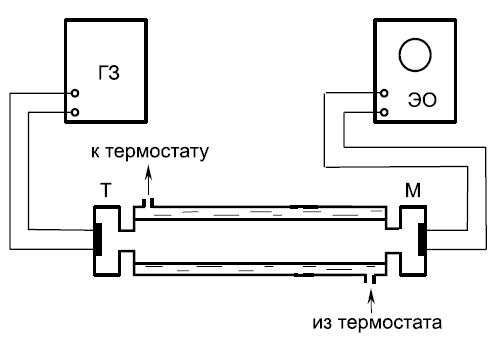
\includegraphics[width=0.6\textwidth]{установка.png}
\label{ris:image}
\end{center}

Звуковые колебания в трубе возбуждаются телефоном Т и улавливаются микрофоном М. Возникающий в микрофоне сигнал возникает на экране осциллографа ЭО.

Установка содерджит теплоизолированную трубу постоянной длины. Воздух в трубке нагревается водой из термостата. Температура газа принимается равной температуре омывающей трубу воды. 

\section{Измерения}

1) Включу все оборудование и убежусь в его работоспособности

Также проверю, что напряжение на генераторе позволяет возбуждать синусоидальный сигнал на осциллографе.

2) Произведу предварительные замеры:

Эффективная длина трубки $L = (740 \pm 1)$ мм

Комнатная температура $T = 22.6 ^\circ C = 295.8 K$

3) Резонансную частоту буду определять максимальной амплитудой синусоидального сигнала на осциллографе

Приведу таблицу частот резонансов различных порядков от температуры

\begin{center}
\begin{tabular}{|c|c|c|c|c|}
\hline & \multicolumn{4}{|c|}{$T$, К;   $\nu$, Гц} \\ \hline
N &	295.8	& 313.2	& 328.2	& 338.2	\\ \hline
1 & 250		& 255	& 260	& 265	\\
2 & 475		& 489	& 500	& 509	\\
3 & 700		& 725	& 740	& 750	\\
4 & 930		& 955	& 980	& 995	\\
5 & 1158	& 1190	& 1220	& 1240	\\
6 & 1388	& 1430	& 1465	& 1490	\\
7 & 1618	& 1670	& 1705	& 1730	\\
\hline
\end{tabular}
\end{center}

\section{Обработка}

Построю графики зависимости частоты резонанса от их номера

\begin{center}
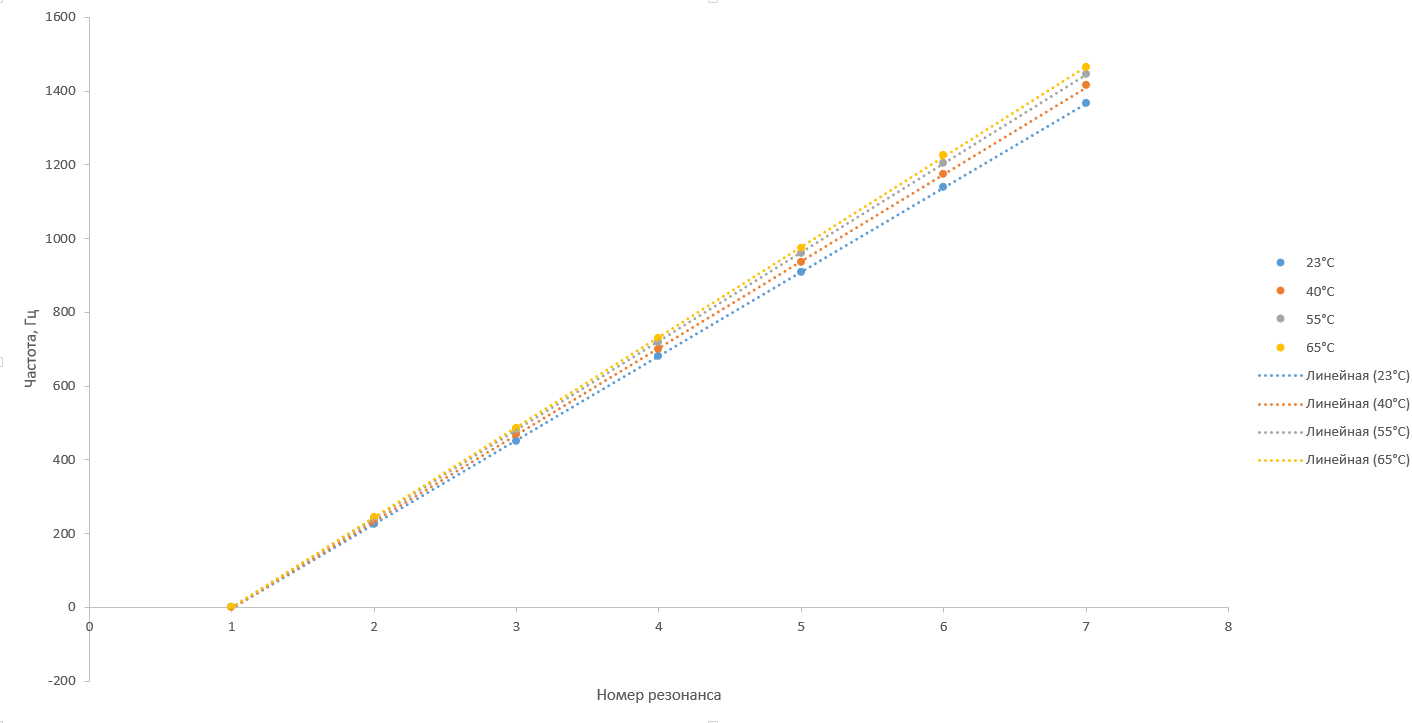
\includegraphics[width=1\textwidth]{график.png}
\label{ris:image}
\end{center}

Найду угловые коэффициенты прямых для каждой температуры по МНК.

\[
	a = \frac{n \sum_{i=1}^n N_i \nu_i - \left( \sum_{i=1}^n N_i \right) \left( \sum_{i=1}^n \nu_i \right)}{n \sum_{i=1}^n N_i^2 - \left( \sum_{i=1}^n N_i \right)^2}
\]

\[
	b = \frac{\sum_{i=1}^n \nu_i - a \sum_{i=1}^n N_i}{n}
\]

Также рассчитаю их погрешности

\begin{equation}
	S_a^2 = \frac{\sum_{i=1}^n N_i^2}{n \sum_{i=1}^n N_i^2 - \left( \sum_{i=1}^n N_i \right)^2} \cdot \frac{\sum_{i=1}^n \left( \nu_i - b - a \cdot N_i \right)^2}{n - 2}
\end{equation}

\begin{center}
\begin{tabular}{|c|c|}
\hline T, K & a, Гц \\ \hline
295.8	& $(228.14 \pm 0.45)$ \\
313.2	& $(235.43 \pm 0.69)$ \\
328.2	& $(240.89 \pm 0.31)$ \\
338.2	& $(244.54 \pm 0.48)$ \\
\hline
\end{tabular}
\end{center}

Запишу итоговую связь для показателя адиабаты

\begin{equation}
	\boxed{\gamma = \frac{4 \mu L^2 a^2}{RT}}
\end{equation}

Его погрешность составит

\begin{equation}
	\varepsilon_\gamma = \varepsilon_T + 2 \varepsilon_a + 2 \varepsilon_L
\end{equation}

И, наконец, составлю таблицу

\begin{center}
\begin{tabular}{|c|c|}
\hline T, K & $\gamma$ \\ \hline
295.8	& $(1.344 \pm 0.009)$ \\
313.2	& $(1.352 \pm 0.012)$ \\
328.2	& $(1.351 \pm 0.008)$ \\
338.2	& $(1.351 \pm 0.009)$ \\
\hline
\end{tabular}
\end{center}

Наконец найду среднее значение показателя адиабаты

Его погрешность состоит из случайной погрешности выборки и погрешности каждого её элемента

\begin{equation}
	\Delta_\gamma = \sqrt{\Delta_\text{приб}^2 + \Delta_\text{случ}^2}
\end{equation}

\begin{equation}
	\boxed{\gamma_0 = (1.350 \pm 0.011)}
\end{equation}




\section{Вывод}

В данной лабораторной работе был проверен метод нахождения показателя адиабаты воздуха, основанный на теоретических сведениях о его связи со скоростью звука. Хорошее совпадение показателя адиабаты с табличным значением подтверждает работоспособность экспериментальной установки, основанной на возбуждении стоячих волн в воздухе при разной температуре.

Также эксперимент подтверждает малую зависимость(в пределах погрешности) показателя от температуры, при её значениях, близких к комнатным.

\end{problem}
\end{document}